\chap{Приложение B: Моделирование антенной решётки}
\setcounter{chapter}{2}
\setcounter{figure}{0}

Перенесём данные в MATLAB и проведём дополнительные рассчёты.
 На Рис. \ref{fig:system-diagram-x} и \ref{fig:system-diagram-y} показаны ДН для плоскостей oXZ и oYZ ($\phi_{x,y}=0, 90^\circ$) для углов $\theta_0=-18^\circ, 0^\circ, 18^\circ$. Для наглядности на них приведены ДН излучателя, нормированные к $K_y$ системы. 

\begin{figure}[H]
	\centering
	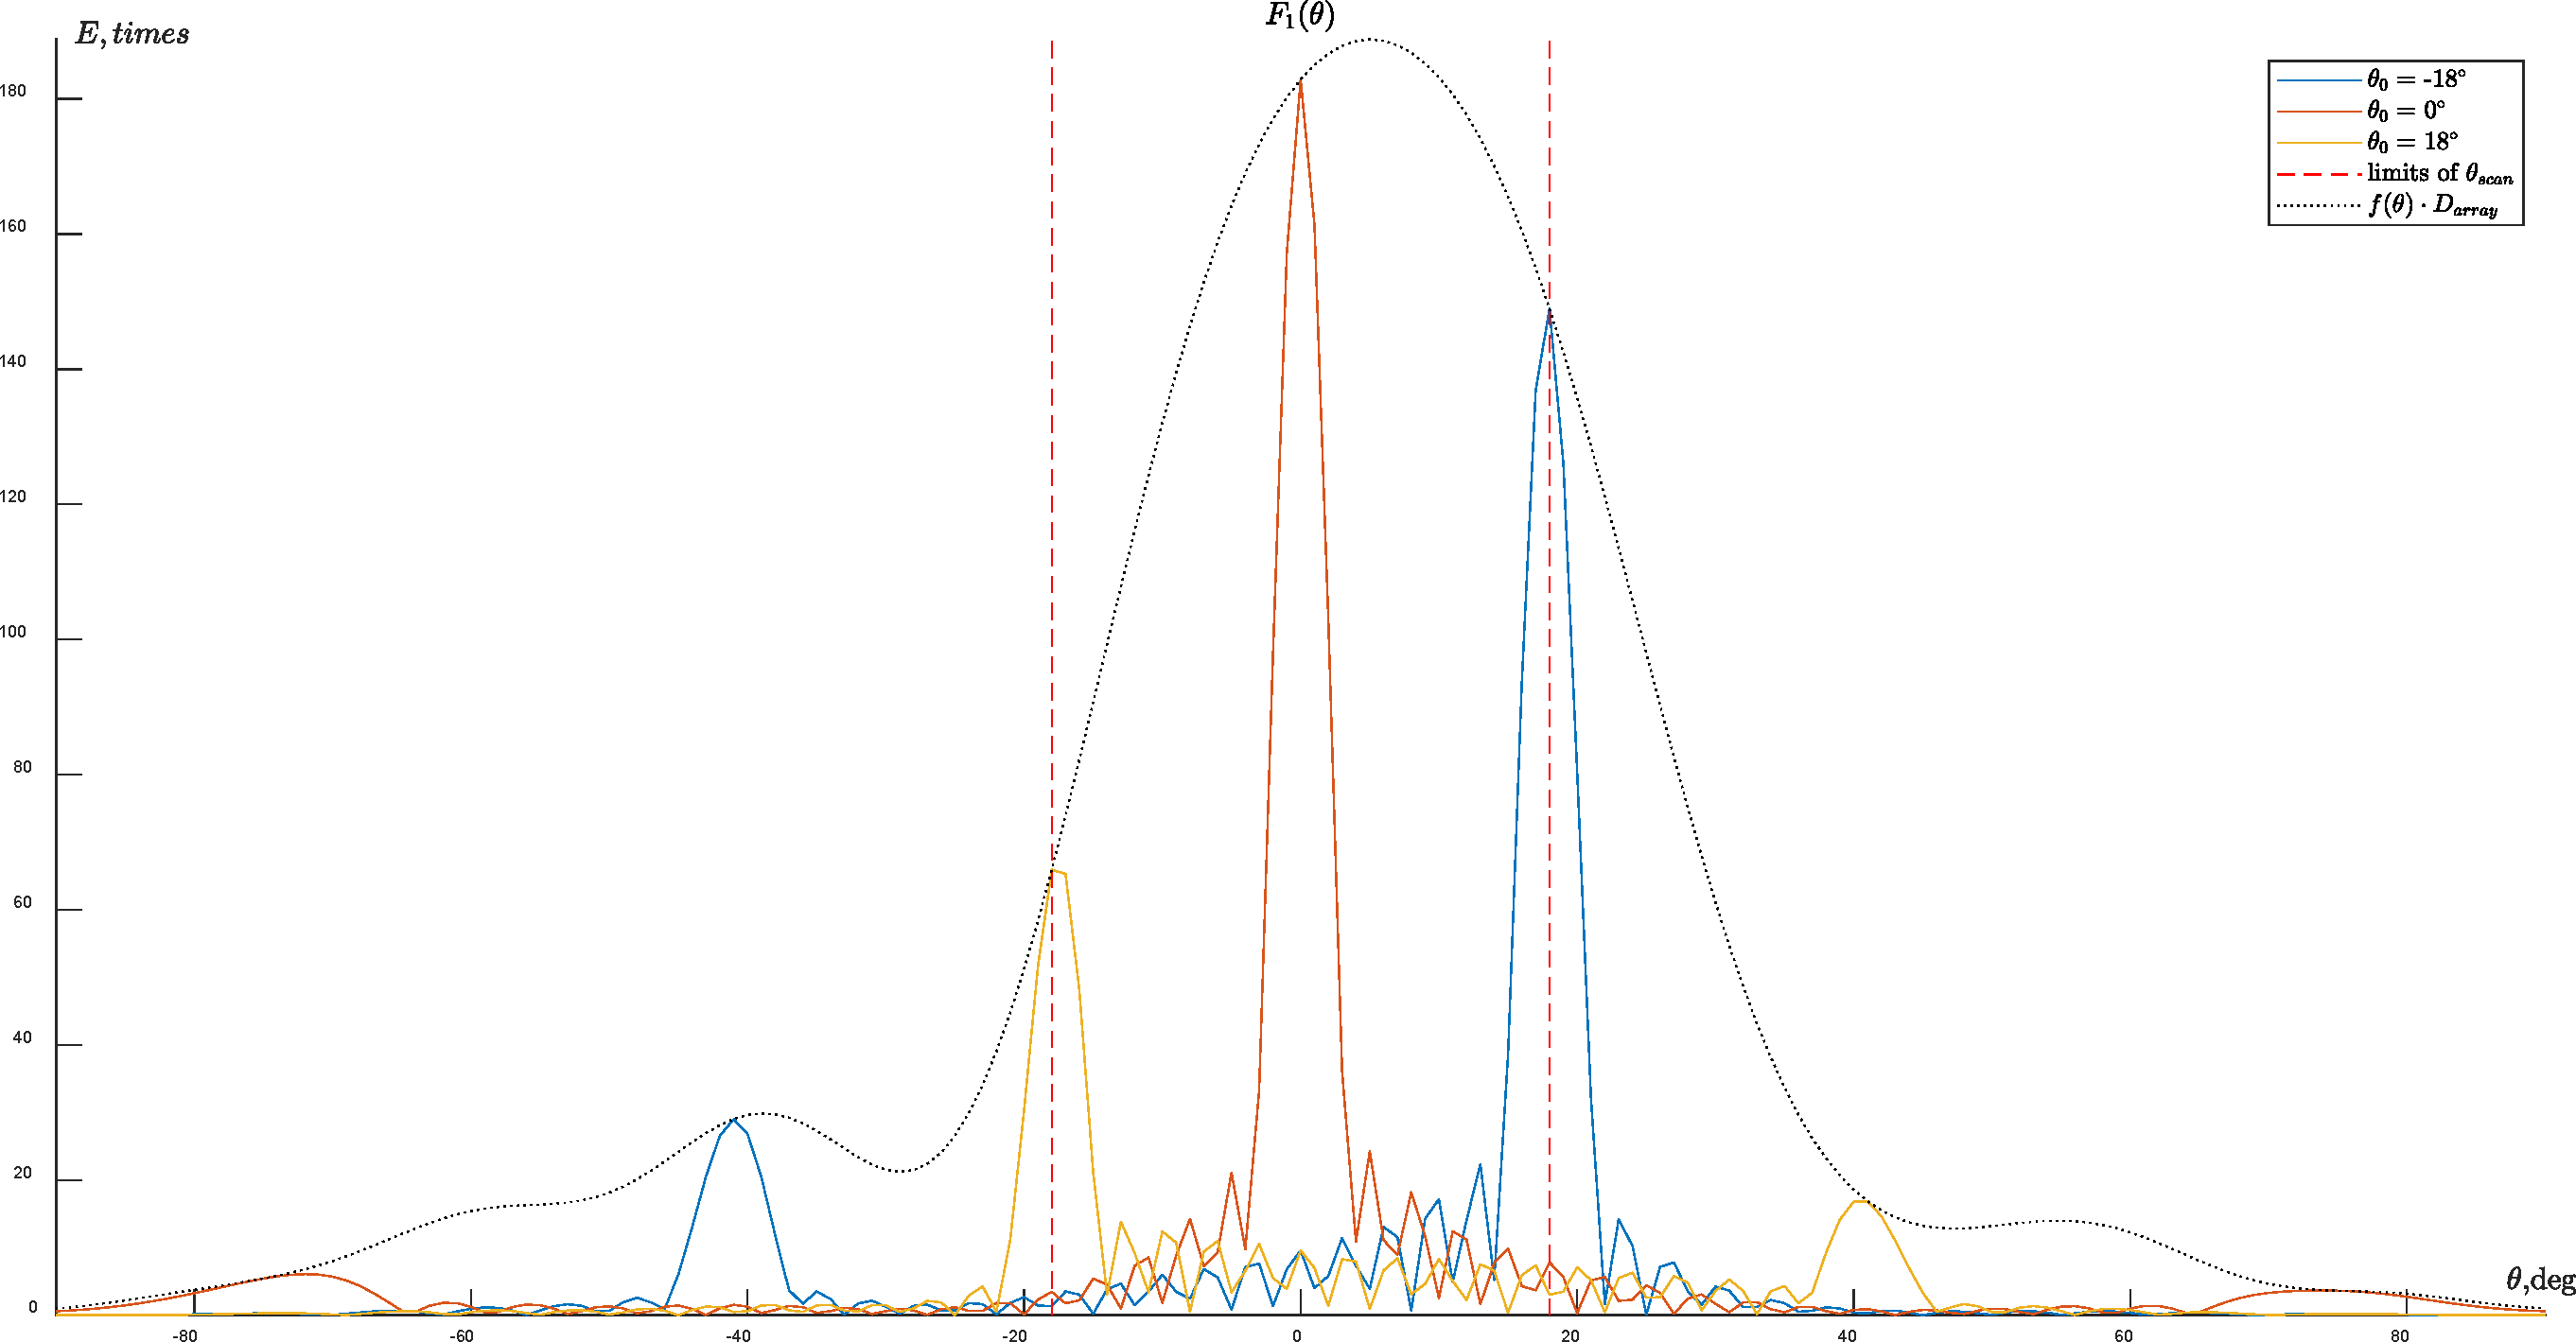
\includegraphics[width=0.9\textwidth]{system-diagram-x.pdf}
	\caption{ДН системы в плоскости oXZ}
	\label{fig:system-diagram-x}
\end{figure}

\begin{figure}[H]
	\centering
	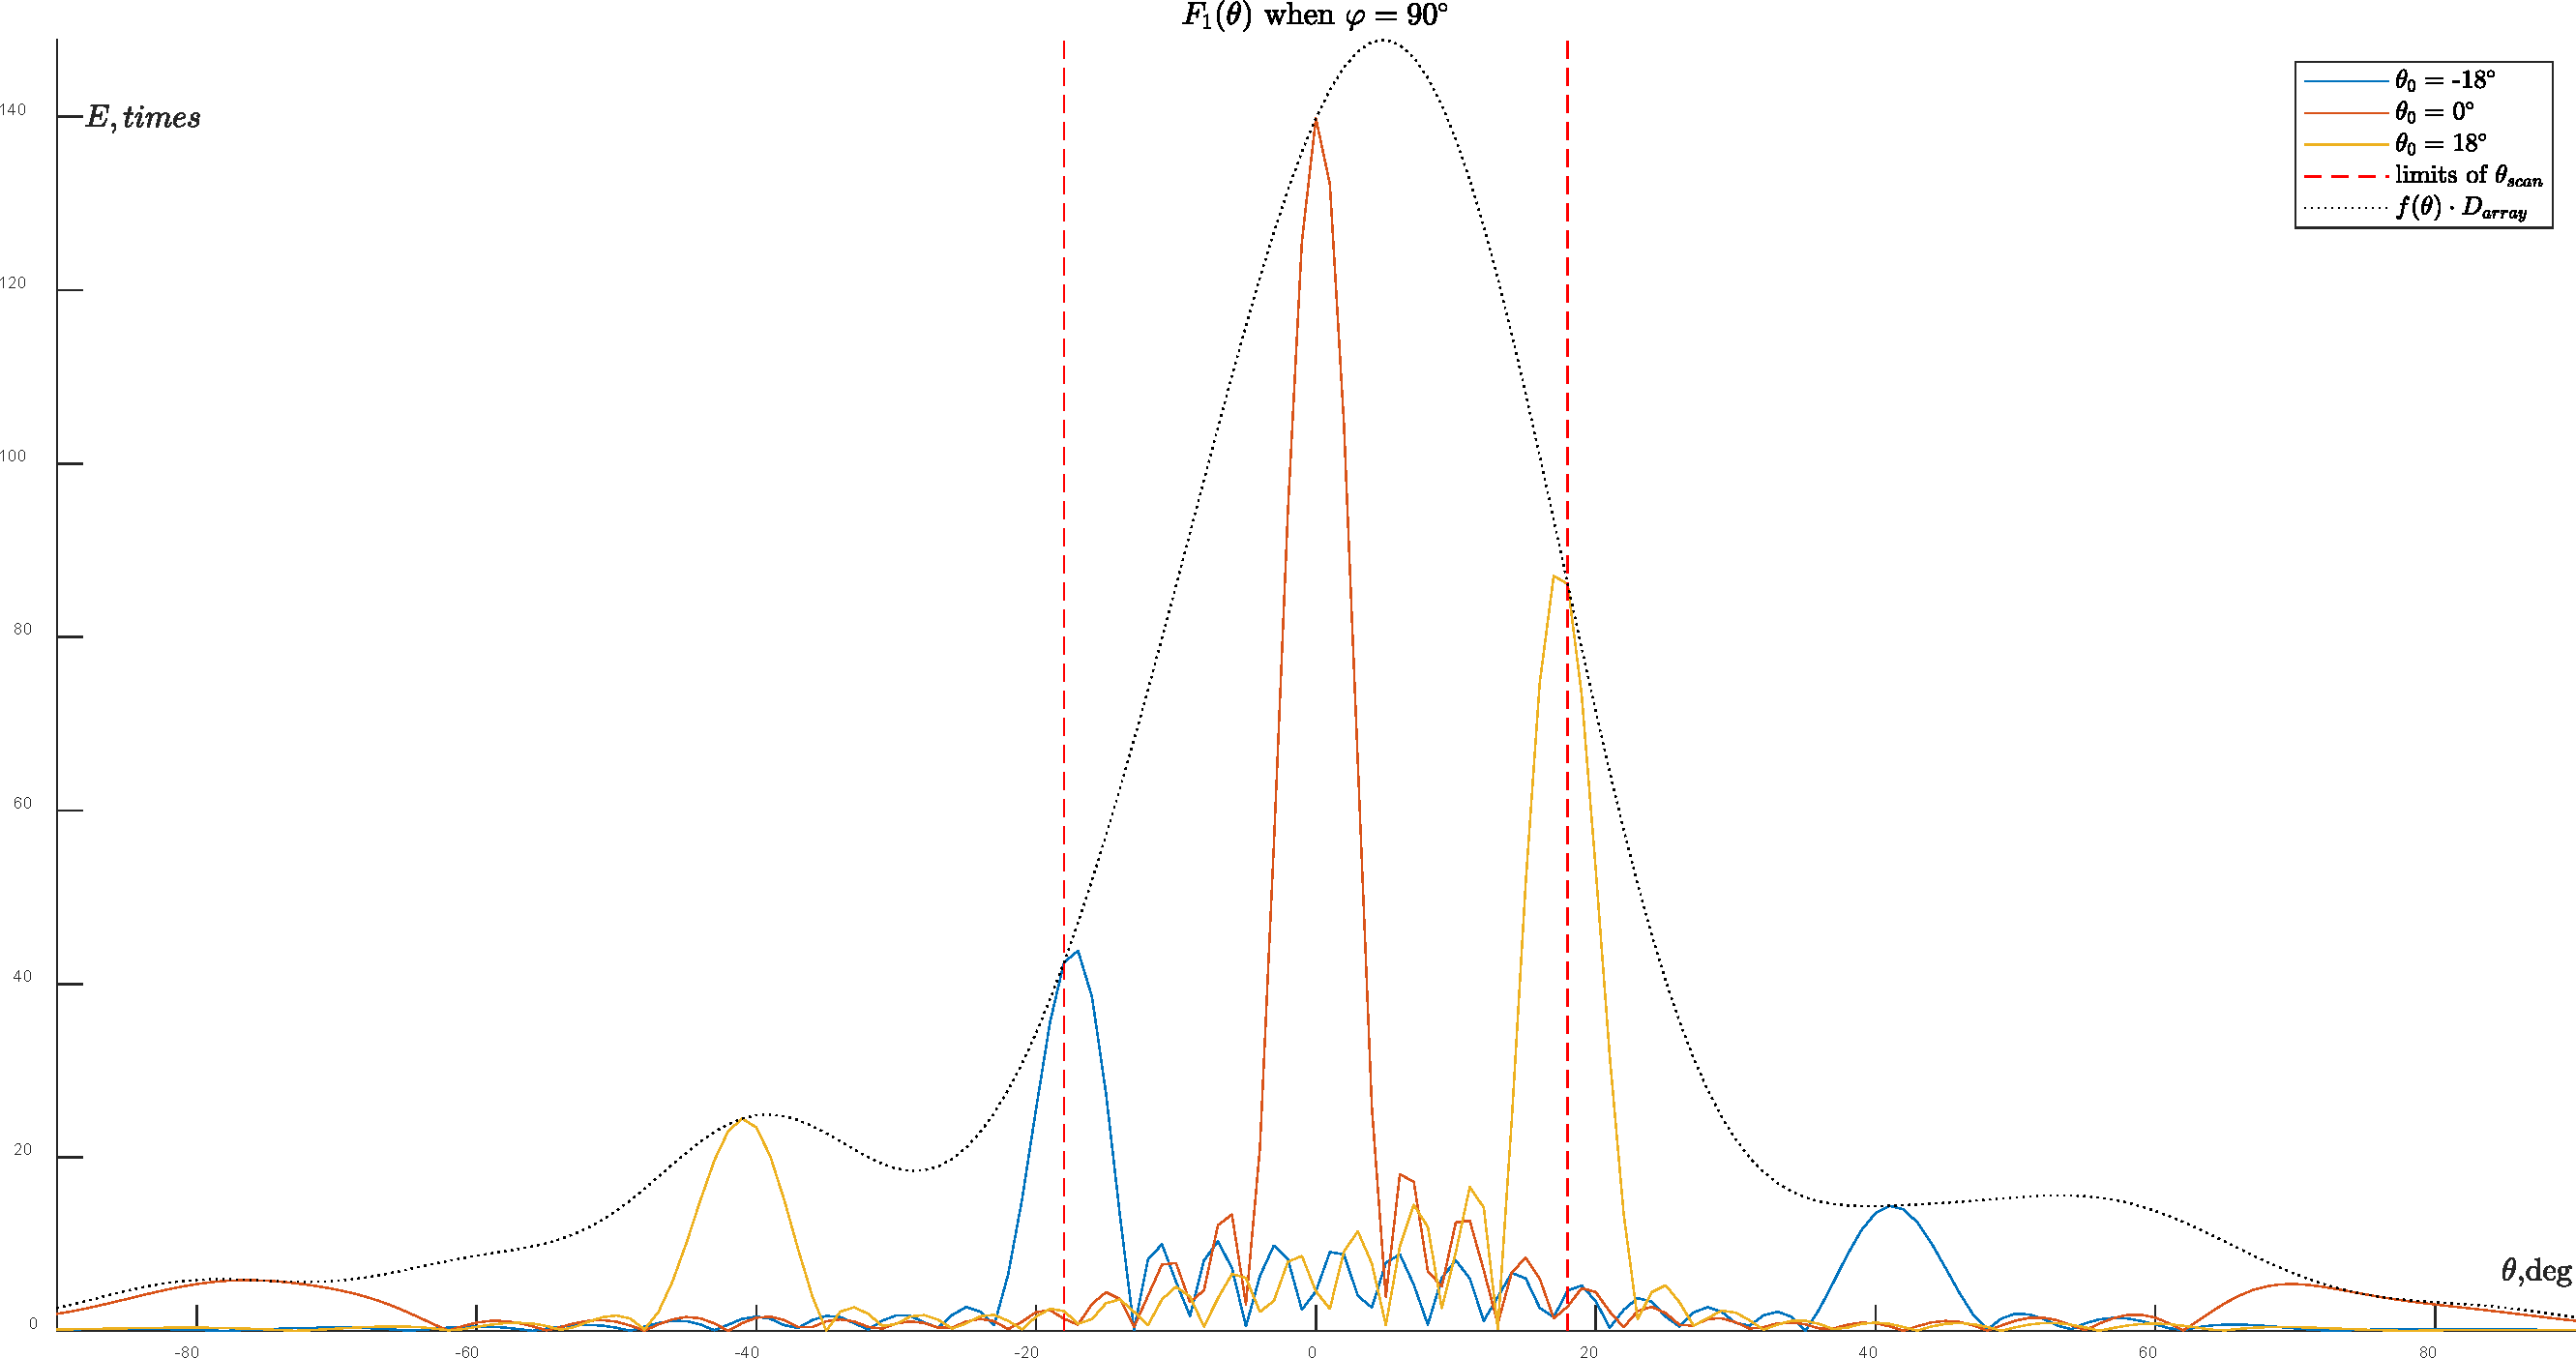
\includegraphics[width=0.9\textwidth]{system-diagram-y.pdf}
	\caption{ДН системы в плоскости oYZ}
	\label{fig:system-diagram-y}
\end{figure}